\documentclass{article}

\usepackage[LGR, T1]{fontenc}
\usepackage[utf8]{inputenc}
\usepackage[greek]{babel}
\usepackage{setspace}
\usepackage{amsmath}
\usepackage{graphicx}
\usepackage{caption}
\usepackage{subfiles}
\usepackage{graphicx}
\usepackage{subfig}
\graphicspath{ {./data/} }

\title{2η Εργασία Στο Μάθημα Της Αριθμητικής Ανάλυσης}
\doublespacing
\author{ Ονοματεπώνυμο : Παπαδόπουλος Αναστάσιος \\
            ΑΕΜ : 3654 \\
            Διδάσκων : Τέφας Αναστάσιος }

\begin{document}
\normalsize
\maketitle
\vspace{15px}
\begin{center}
    \centering
    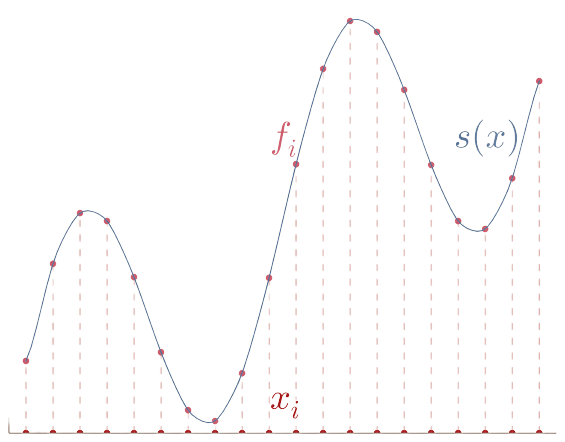
\includegraphics[scale=2.8]{intro_page_logo.png}
\end{center}
\begin{figure}[b]
    \begin{center}
        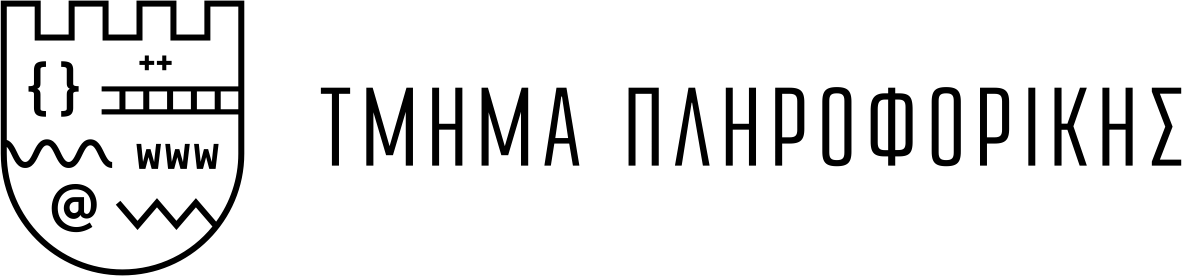
\includegraphics[scale=0.15]{csd_logo.png}    
    \end{center}
\end{figure}
\newpage
\doublespacing
\tableofcontents
\newpage

% Intro page
\subfile{intro.tex}

% Exercise 5
\subfile{./Exercise5/exercise5.tex}
\subfile{./Exercise5/polynomial.tex}
\subfile{./Exercise5/splines.tex}
\subfile{./Exercise5/leastSquares.tex}
\subfile{./Exercise5/comparison.tex}

% Exercise 6
\subfile{./Exercise6/exercise6.tex}

% Exercise 7
\subfile{./Exercise7/exercise7.tex}
\subfile{./Exercise7/auto_hellas_stock.tex}
\subfile{./Exercise7/hellenic_petroleum_stock.tex}

\end{document}